\documentclass[12pt]{article}
\usepackage[margin=1in]{geometry}
\usepackage{paracol}
\usepackage{titlesec}
\usepackage{setspace}
\singlespacing
\titleformat*{\section}{\fontsize{14}{17}\selectfont\bfseries}
\titleformat*{\subsection}{\fontsize{14}{17}\selectfont\bfseries}
\usepackage{pdfpages}
\usepackage{graphicx}
\graphicspath{{./images/}}
\renewcommand{\thesubsection}{\alph{subsection})}
\usepackage{enumitem}
\usepackage[hyphens]{url}
\usepackage{hyperref}
\setlength{\intextsep}{-5pt}
\begin{document}
\section*{Device Overview}
\begin{paracol}{2}
    \begin{figure}[h]
        \centering
        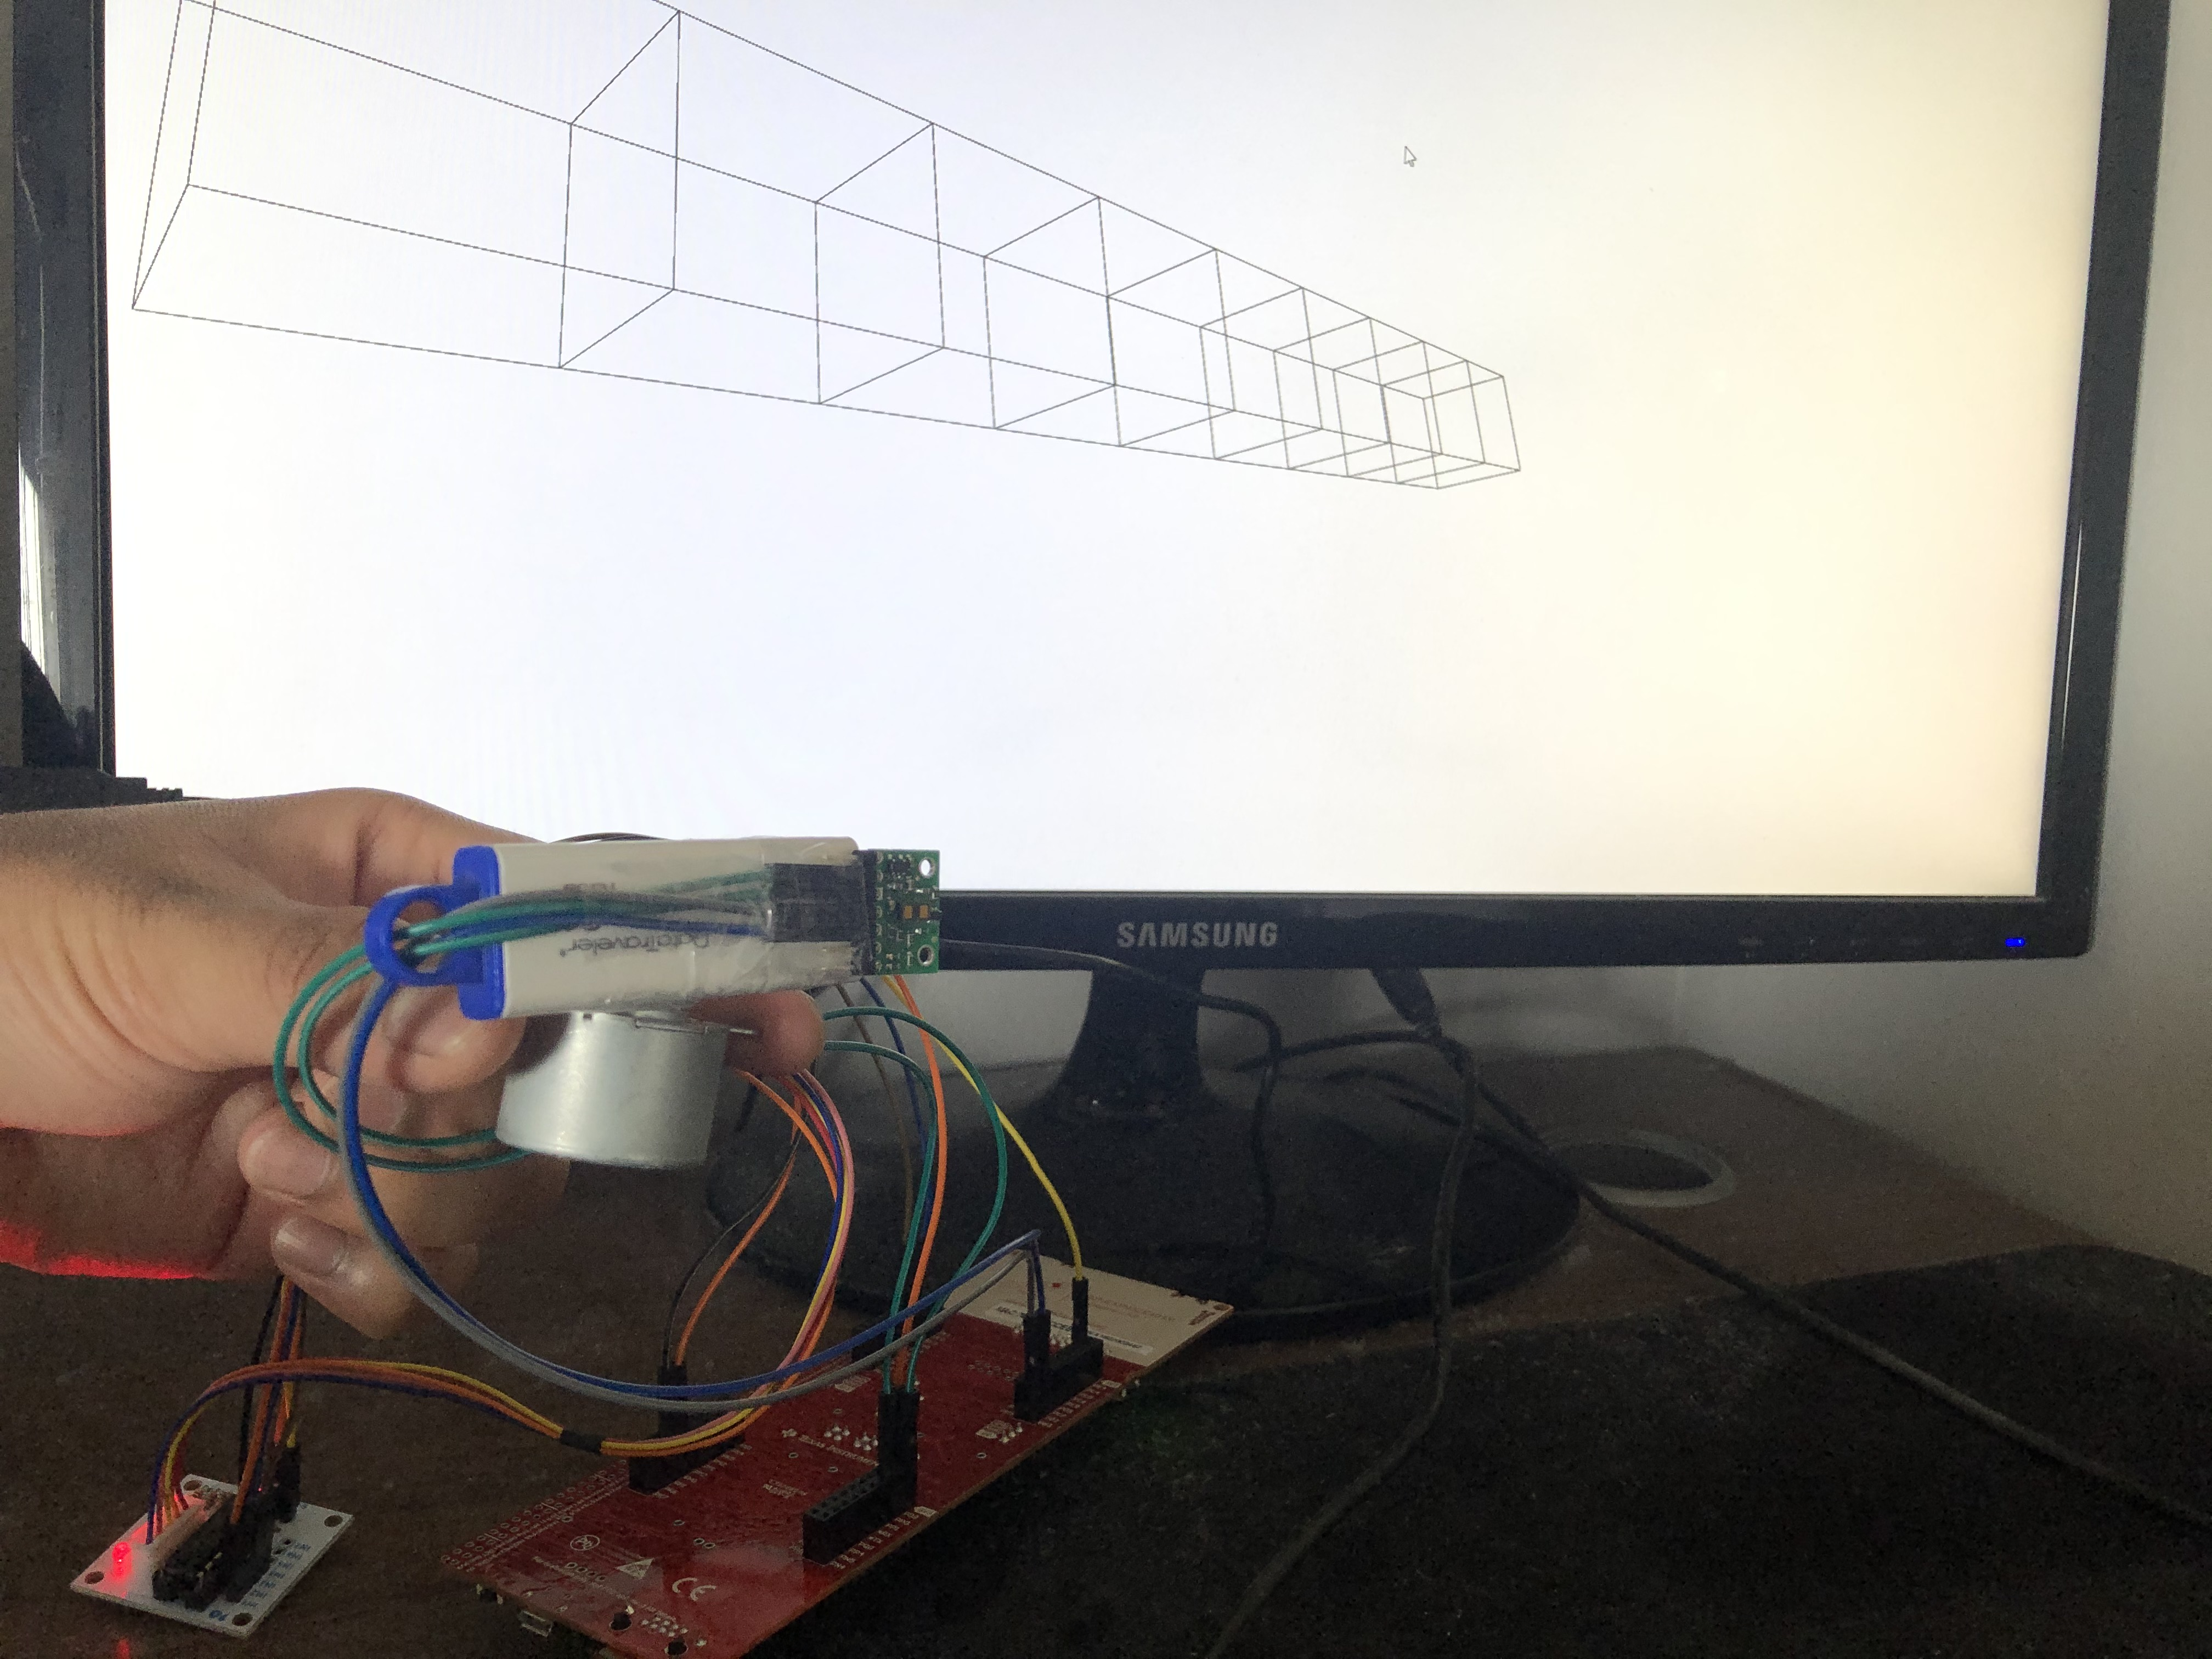
\includegraphics[width=0.45\textwidth]{SystemOverview.jpg} 
        \label{fig:SystemOverview}      
    \end{figure}
    \subsection*{Features}
    %Why do we need it? What does it do? 
    %Act as if your reader has no idea which ToFand microcontroller you are using 
    %Introduce the hardware!
    \begin{itemize}[nosep]
        \item Integrated Lidar system 
        \begin{itemize}[nosep]
            \item 360 degree distance measurements within single plane
            \item Orthogonal displacement samples
            \item Data communication via USB
            \item 3D visualization of data
        \end{itemize} 
        \item Texas Instruments MSP432E401Y Microcontroller 
        \begin{itemize}[nosep]
            \item Arm Cortex-M4F Processor Core 
            \item 96 MHz bus speed
        \end{itemize}
        \item UNL2003 Stepper Motor Controller
        \begin{itemize}[nosep]
            \item 512 steps for 360 degree rotation
            \item LED state indictators
            \item 5V-12V operating voltage
        \end{itemize}
        \item VL53L1X Time-of-Flight Sensor
        \begin{itemize}[nosep]
            \item Accurate distance measurements \\ ($\pm$20 mm ranging error)
            \item Up to 4m range
            \item 2.6V-3.5V operating voltage
        \end{itemize}
        \item Data communication
        \begin{itemize}[nosep]
            \item I$^2$C serial communication between MSP432E401Y and VL53L1X
            \item UART serial communication\\ between MSP432E401Y and PC \\ supported via Python
        \end{itemize}
        \item Visualization
        \begin{itemize}[nosep]
            \item 3D visualization of mapped data
            \item Open3D python library for 3D\\ data processing
            \item Supported on Python 3.6
        \end{itemize}
    \end{itemize}
    \switchcolumn
    %\setcounter{subsection}{1}
    \subsection*{General Description}

    \indent \indent The 2DX4 Final Project Lidar system is an integrated 3D scanning system that is capble of recording distances in multiple 360 degree planes along an orthogonal axis and process the recorded data to produce a 3D visualization of the space that was mapped.

    The system is comprised of a microcontroller, a stepper motor and a time-of-flight sensor. The microcontroller is responsible for managing all operations of the system excluding 3D visualization, providing power to other components of the system, and transmitting all recorded data to an external device through serial communication. The stepper motor allows for the system to have a 360 degree range of motion, allowing for the mounted time-of-flight sensor to record distance measurements in the a full vertical plane.
    
    The VL53L1X ToF sensor emits pulses of infrared laserlight, determining distances to objects by measuring the time laser pulses take to be reflected back to a detector. The sensor calculates the distance using this timing data based on its configuration settings, and transmits this data to the microcontroller through I$^2$C.

    The system connects to a PC, running the included python scripts. The microcontroller transmits data to the PC via UART, sending status messages and distance measurements. The data is then visualized through the use of an included python script. \\
    
    \begin{figure}[h!]
        \centering
        \fbox{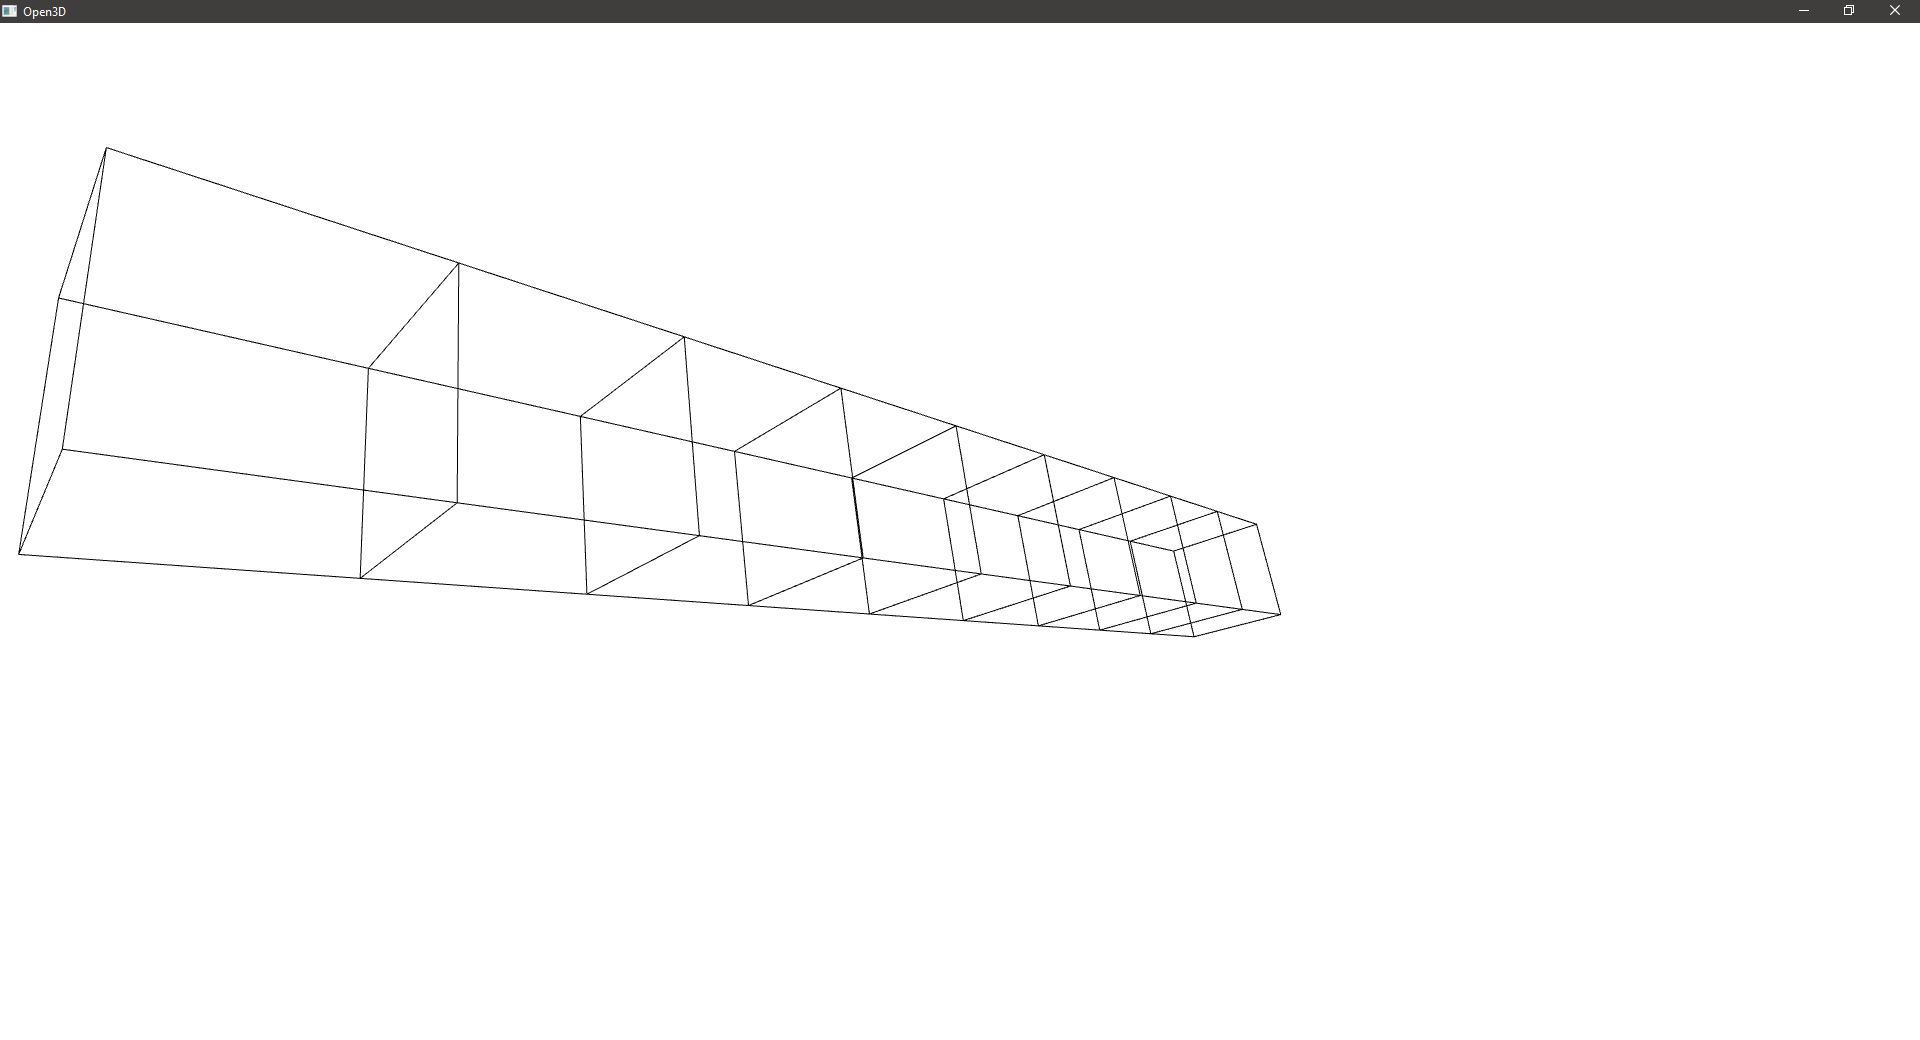
\includegraphics[width=0.45\textwidth]{PCDisplay.png}}
        \label{fig:PCDisplay}
    \end{figure}

\end{paracol}
\newpage
%\setcounter{subsection}{2}
\subsection*{Block Diagram}
\begin{figure}[h!]
    \centering
    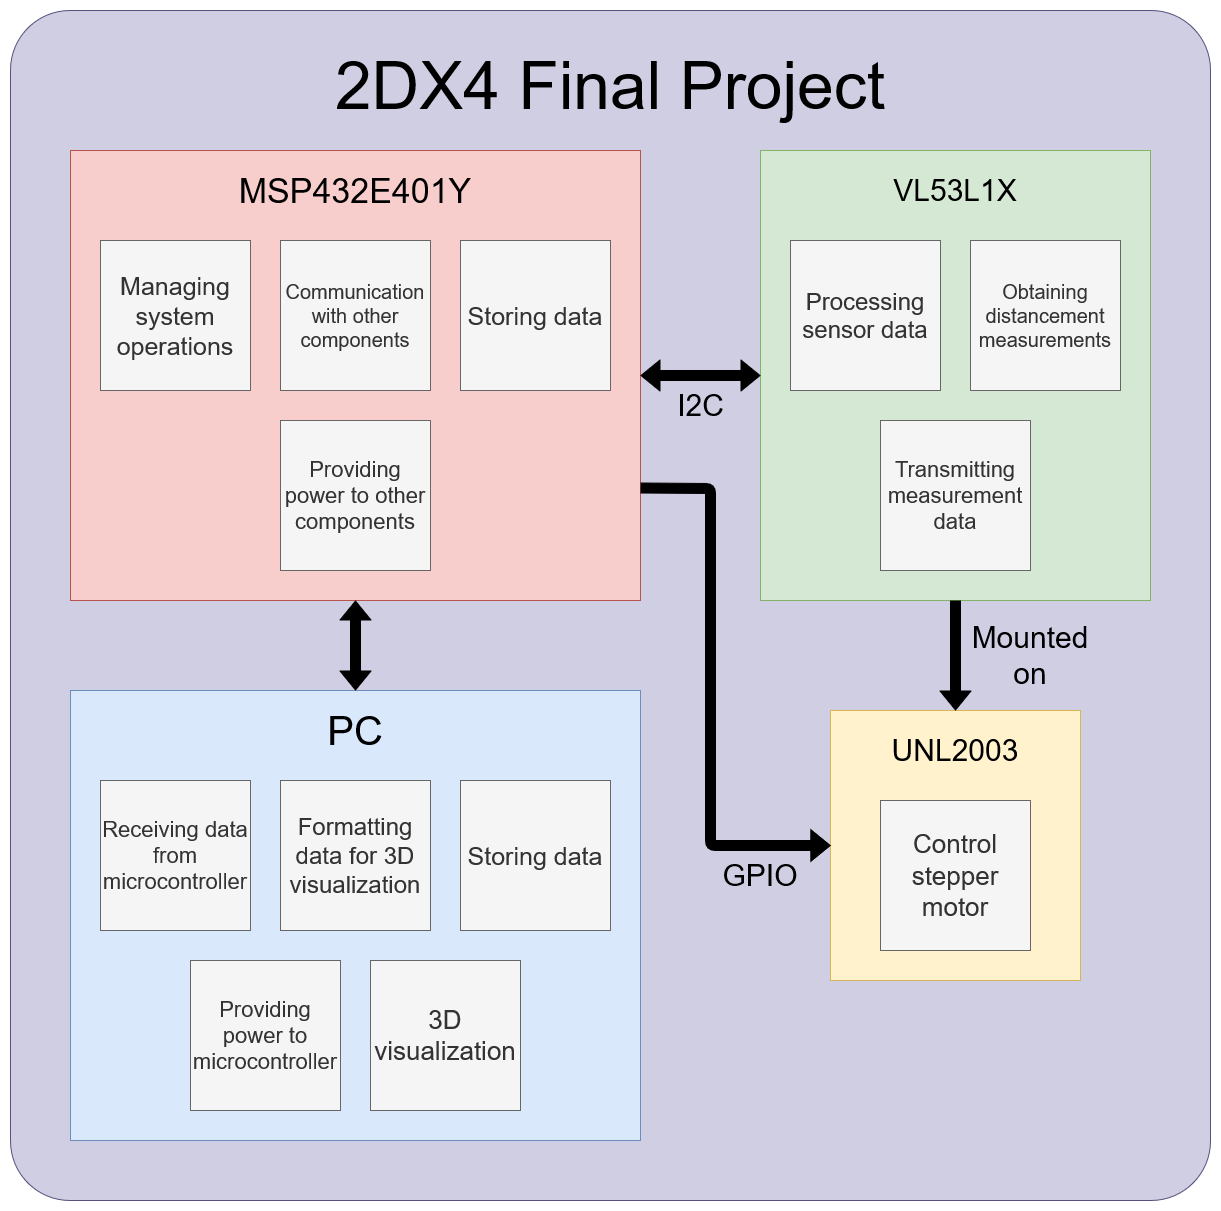
\includegraphics[width=0.75\textwidth]{BlockDiagram.png}
    \caption{Block Diagram}
    \label{fig:BlockDiagram}
\end{figure}
\section*{Device Characteristics}
\begin{table}[h]
    \begin{tabular}{|l|l|l|l|l|l|}
    \hline
    \multicolumn{2}{|c|}{MSP432E401Y}                           & \multicolumn{2}{c|}{UNL2003}                                                                                                                                    & \multicolumn{2}{c|}{VL53L1X}                                                                                                                                   \\ \hline
    \multicolumn{1}{|c|}{Feature} & \multicolumn{1}{c|}{Detail} & \multicolumn{1}{c|}{\begin{tabular}[c]{@{}c@{}}Device \\ pin\end{tabular}} & \multicolumn{1}{c|}{\begin{tabular}[c]{@{}c@{}}Microcontroller\\ pin\end{tabular}} & \multicolumn{1}{c|}{\begin{tabular}[c]{@{}c@{}}Device\\ pin\end{tabular}} & \multicolumn{1}{c|}{\begin{tabular}[c]{@{}c@{}}Microcontroller\\ pin\end{tabular}} \\ \hline
    Bus speed                     & 96 MHz                      & VDD                                                                        & 5V                                                                                 & VDD                                                                       &                                                                                    \\ \hline
    Serial port                   & COM4                        & GND                                                                        & GND                                                                                & VIN                                                                       & 3.3V                                                                               \\ \hline
    Baud rate                     & 115200                      & A                                                                          & PH0                                                                                & GND                                                                       & GND                                                                                \\ \hline
    Distance status               & PN0                         & B                                                                          & PH1                                                                                & SDA                                                                       & PB3                                                                                \\ \hline
    Displacement status           & PL1                         & C                                                                          & PH2                                                                                & SCL                                                                       & PB2                                                                                \\ \hline
                                  &                             & D                                                                          & PH3                                                                                & XSHUT                                                                     &                                                                                    \\ \hline
                                  &                             &                                                                            &                                                                                    & GPIO1                                                                     &                                                                                    \\ \hline
    \end{tabular}
\end{table}
\newpage
\section*{Detailed Description}
\subsection*{Distance Measurement}
%The Transducer/ Precondition Circuit/ ADC are all in the ToF(done for you)
\indent \indent Distance measurements are performed by the VL53L1X Time-of-Flight sensor, taking a measurement every step of the stepper motor as the motor performs a full rotation. This allows the ToF sensor to measure distances in a full 360 degree plane.

%You can describe how the ToFworks
The VL53L1X ToF sensor emits pulses of infrared laser light which are reflected off objects in the laser's field of view. The sensor measures the time it takes for the emitted pulses of infrared laser light to be reflected to one of its detectors after having reached a nearby object.  The sensor calculates the distance by using the acquired timing data based on its configuration settings of the sensor, and then transmits this data to the microcontroller through the I$^2$C serial communication protocol.

The ToF settings used in the initialization of the sensor are the default configuration settings provided in the VL53L1 Core API. All ToF functions that are used in the system are provided in the VL53L1 Core API  distributed by STMicroelectronics or in the platform code provided by the course coordinator, and implementation of all functions remains unmodified from the code provided.

%You want to discuss the whole process from acquisition, to transmission, to conversion into the xyzplane
The entire process from the acquisition of distance measurement data to visualization the other in 3D is outlined in the flowchart in Figure \ref{fig:Flowchart}. In the initial microcontroller initialization process, the I$^2$C capabilities of the microcontroller are initialized, allowing the microcontroller to communicate with the Tof sensor. All necessary variables that will be used for ToF functions are also initialized. The ToF sensor is be booted and initialized and then waits for a button press to begin data capture.

An interrupt-based button system is used to start and stop data capture for the ToF sensor. The current state of the lidar system is stored in the variable \texttt{int state}, which is 0 when the system is not capturing data and 1 when the system is capturing data. Pressing a button on the microcontroller will trigger an interrupt that will change the value of \texttt{int state}. The functions of the system generally exist in two loops (one for data capture, another to prompt the user to begin data capture) which always check the value of \texttt{int state} at the end of the loop. When the state is changed, the program will exit the loop and enter the other loop.

When the system is in the data capture state, the ToF sensor begins ranging, and then enters a loop for an entire stepper motor rotation. At the start of the loop, the program waits for the sensor data to be ready, and extracts the necessary information when the the data is ready. This data is then transmitted to the microcontroller through the sensor's I$^2$C functions. The data is stored in the microcontroller and transmitted to the PC through UART, and this distance measurement data is processed by the PC through the \texttt{data\_collection.py} python script to write the data into a \texttt{.xyz} file. After the data transmission, the stepper motor moves one step. If the button interrupt is trigger inside the loop, or 512 distance measurements (one motor rotation is comprised of 512 steps) have been taken, the ToF sensor ends ranging, entering the loop that prompts the user to press the button to restart data capture.

%You will want to use formulas (define them) and give examples of their use
The python script, \texttt{data\_collection.py}, receives the data sent via UART from the microcontroller by using the \texttt{pySerial} library, and processes the data measurements to write them to an \texttt{.xyz} file. The x-component of the data is discussed in the displacement measurement section. The y and z-components of the data are calculated using the distance measurements by applying simple trigometric functions on the data. The angle that the motor has turned can be determined by simplying counting the number of steps performed, dividing by the number of steps in a rotation, and multiply by 2$\pi$ radians. The y and z-components can be determined by multiplying the distance measurement by the appropriate trigometric function (the argument of the function is the angle). Assuming the initial state of the ToF sensor is facing up, the y-component is the distance multipled by the cosine of the angle ($y = d\cos{\theta}$) and the z-component is the distance multipled by the sine of the angle ($z = d\sin{\theta}$). 

Only two full sets of data were able to be collected due to mechanical issues with the mounting mechanism. The second set of data has some errors in the data due to these mechanical issues, causing a subsection of the data to have incorrect distance measurement values. The data collected using the sensor distance measurements can be found as \texttt{2dx4data.xyz} in the "Program" folder.
\subsection*{Displacement Measurement}
%You will also need to discuss how you actually implemented displacement in your project
\indent \indent The displacement measurement is currently modified by manually changing the value of the x-displacement in the \texttt{data\_collection.py} python script. This x-displayment will automatically be reflected in the \texttt{.xyz} file produced by the python script. As the x-displacement is manually measured, there is no modification that needs to be done by the program on the values entered before entering them into the \texttt{.xyz} data file.

%You will need to explain how you would have completed your design to measure displacement using the IMU sensor
If the project were to be completed with the addition of the IMU sensor, the design of the lidar system would largely remain unchanged, with the only modifications being the inclusion of the external displacement LED, the integration of the IMU's displacement measurement system to determine the x-displacement instead of requiring manually measurements, and a displacement-based interrupt system that would automatically begin data capture after a certain amount of displacement has been acheieved.

The microcontroller would transmit displacement information along with distance measurements during data collection, and these would be implemented into the python script \texttt{data\_collection.py} to adequately adjust the values produced in the \texttt{.xyz} file.
\subsection*{Visualization}
%Control/ Communicate
\indent \indent 3D visualization of data is performed by importing the data in the \texttt{.xyz} file format into Python through the use of the Open3D library, and then using the library's functions to visualize the data. 

%Introduce the computer and the program you are using!
%OS, computer specs, program version etc
The 3D visualization was tested on a Dell Inspiron 7370 Windows 10 laptop running Windows 10 Home Version 1909. The laptop featured a quad-core Intel i7-8550U CPU, an integrated Intel UHD Graphics 620 graphics chipset, and 8 GB of dual-channel DDR4 memory running at 2400 MHz. All Python code was from inside Visual Studio Code Version 1.44.0. The data collection python script, \texttt{data\_collection.py}, was run on Python 3.8.2 while the \texttt{open3d\_visualization.py} python script had to be run on Python 3.6.8 due the \texttt{Open3D} library's lack of Python 3.8 support.

%How did you do it?
%What functions/ libraries did you use?
%How is the data stored and processed?
%How does it visualize (refer to lecture slides)
%Do not copy and past your code! Paragraph describing how you did it!
The visualization was done through the use of the open-source \texttt{Open3D} Python library, which includes functions to read and format data in an appropriate format for visualization. 3D visualization imported data that was stored in the \texttt{.xyz} file format and processed the data to be compatible with the library. Once the data was ready to be used by the library, a point cloud was created using an \texttt{Open3D} function, the point cloud contains all the points in that will be present in the visualization. The point cloud is also used to create a line set which contains all points in the point cloud, as well as the lines that will be present in the visualization. The lines contain all individual points in a slice, with several lines connecting two slices together. Once the line set is created, the library's visualization function can be used to draw the points and lines present in the line set and visualize them. The procress of visualization is shown towards the end of the flowchart in Figure \ref{fig:Flowchart}.

Only two full sets of data were able to be collected due to mechanical issues with the mounting mechanism as mentioned in the distance measurement section. The errors in the second set of data causes a subsection of the data to appear almost as a straight line due to incorrect distancement measurements being taken. The data collected using the sensor distance measurements can be found as \texttt{2dx4data.xyz} in the "Program" folder.
%Refer to your flowchart to describe the process
\section*{Application Example}
%Walk us through an application of acquiring signal and mapping into using python or other approach
%This can be a numbered list
%1-2 small images can be include if that helps
%How does someone set up and use your device?
%Step by step guide 
%Particular focus is on communication protocol (COM port settings, baud rate etc.) if used
%Allows someone else to set up your device without you being present
In order to the use the integrated lidar system, there is a setup process to ensure that the user has all the necessary software installed on their computer. This setup process is necessary for the user's PC to be able to receive data from the lidar system and also to be able to visualize the data. The steps in the setup process on Windows 10 machines are:
\sloppy
\begin{enumerate}
    \item Download the appropriate XDS Emulation Software for your operating system from \url{https://software-dl.ti.com/ccs/esd/documents/xdsdebugprobes/emu_xds_software_package_download.html}. Run the setup executable and complete setup using the "Typical" setup option. This will allow the user to debug the microcontroller and communicate with microcontroller through the XDS110 UART port.
    \item Download and install a release of Python 3.6. The latest release can be downloaded from \url{https://www.python.org/downloads/release/python-368/}. Run the setup, however ensure to select the "Add Python 3.6 to path" when prompt to customize your installation. The installation can be performed with the default installation settings.
    \item After Python installation, open command prompt in administrator mode by searching "Command Prompt" from the search menu, and right-clicking the icon and selecting "Run as administrator." From the command prompt, you will install the necessary Python libraries, \texttt{Open3D} and \texttt{pySerial}. To do this, simply enter \texttt{pip install open3d} and wait for a confirmation saying all packages have been installed correctly. Similarly, type \texttt{pip install pyserial} to install the \texttt{pySerial} package.
    \item An IDE to edit and run Python files will be necessary. The IDLE integrated development environment included in the default Python installation will be able to perform all the necessary tasks.
\end{enumerate}
\fussy
After setup, your PC has all the necessary software to interact with the lidar system and use all its features. Now you are ready to begin collecting data and visualizing the data. The steps in this process are:
\begin{enumerate}
    \item Open the \texttt{data\_collection.py} python file in an IDE of choice. The IDLE IDE installed during Python installation is adequate and can be accessed by right-clicking the file and selecting the "Edit with IDLE" option. In the IDE, you will be able to change certain parameters of the system.
    \begin{itemize}[noitemsep,topsep=0pt]
        \item The initial x-displacement can be changed by editting the variable \texttt{x} in line 9. The value of the x-displacement is in mm.
        \item The increment of the x-displacement can be changed by editting the variable \texttt{increment} in line 10. The value of the increment is in mm.
        \item The file name where the data is being stored can be adjusted on line 7. Change the file name to your desired file name.
        \item The COM port being used must be set on line 4. To determine the COM port being used for UART serial communication, enter your PC's Device Manager and select "Show hidden devices" under View. The COM port can be found in "Ports (COM \& LPT). Change the COM port on line 4 to the one listed by "XDS110 Class Application/User UART."
    \end{itemize}
    \item Once the \texttt{data\_collection.py} python file has been modified, it can be run inside your IDE of choice.
    \item Connect your PC to the microcontroller by using the micro-USB port on the opposite side of the Ethernet port.
    \item Press the button beside the USB port.
    \item Messages will appear in the terminal of your IDE telling you about the status of your lidar system. Read through the messages and wait until you are given a prompt to begin data capture. If no messages appear in the terminal, there is likely an issue with the serial COM settings or with the XDS110 UART driver.
    \item When given the prompt to press a button to begin data capture, you may move your lidar system and PC to the location which you wish to map. It is important to ensure that connections from the microcontroller to the PC and other components of the system do not come loose.
    \item You may align your ToF sensor's starting position to be facing up by continually being and stopping data capture by pressing the GPIO J1 buttno, however this is not completely necessary. If it has a different initial position, the visualization will still be accurate, however the xyz-values recorded will simply be with reference to a different position. For reference, the positive x-axis is the direction of the shaft of the stepper motor, the positive y-axis is in the direction where the ToF sensor is initially facing, and the positive z-axis is rotated 90 degrees clockwise from the y-axis. 
    \item Press the GPIO J1 button to begin data capture, it is important to ensure that no wires become loose or tangled during this stage and that valid distance measurements are appearing on the terminal of your IDE. If the values appear incorrect, there may be issues with the ToF sensor or its connection with the microcontroller.
    \item Once the stepper stops rotating and a message appears in the terminal saying that data capture has ended, you may move to the next position that you want to map based on the increment set in your python file. It is fine to record data from a different displacement that what was stated, however you will need to manually edit the data to reflect this change.
\end{enumerate}
%You must also describe how the x y z plane is defined with respect to your measurements
%In 2DX4 lecture, we have used the y z place for vertical slices and x for the movement forward
Once data collection has been completed, you will want to create a 3D visualization of the recorded data. To achieve this, the \texttt{open3d\_visualization.py} python file is used. The steps in the visualization process are:
\begin{enumerate}
    \item Open and run the \texttt{open3d\_visualization.py} python file in your IDE of choice. You may need to adjust the file name on line 9 in the code if you have adjusted the file name in the \texttt{data\_collection.py} script earlier.
    \item A new window will appear titled "Open3D." This window contains the 3D visualization of your data. You will be able to use your mouse to rotate and zoom in the visualization.
\end{enumerate}
\section*{Limitations}
\begin{enumerate}[label=(\arabic*)]
    \item %Summarize  any  limitations  of  the  microcontroller  floating  point  capability  and  use  of  trigonometric functions.
    The microcontroller has a Floating-Point Unit (FPU) that can support single-precision (32-bit) addition, subtraction, multiplication, division, multiply-and-accumulate, and square root operations. The FPU can also perform conversions between floating-point data formats. Trigonometric functions from the \texttt{math.h} library can be performed on \texttt{float} (single-precision floating-point number) variables, therefore there should be no issues with the use of trigonometric functions.
    \item %Calculate your maximum quantization error for each of the IMU and ToF modules.
    The maximum quantization error for the ToF module is $\frac{4000mm}{2^{16}} = 6.10 \times 10^{-2} \ mm$. The maximum quantization error for the IMU module is $\frac{32g}{2^{16}}=\frac{32\cdot9.81 m/s^2}{2^{16}} = 4.79 \times 10^{-3} \ m/s^2$.  
    \item %What is the maximum standard serial communication rate you can implement with the PC. How did you verify?
    The maximum standard serial communication rate that can be implemented with the PC is 128000 bits per second. This was verified in the PC's device manager, by checking the port settings for the XDS110 UART Port.
    \item %What were the communication method(s) and speed used between the microcontroller and theIMUand ToF modules?
    The communication between the microcontroller and the ToF module uses I$^2$C serial communication with the microcontroller ports used for I$^2$C configured to have a 100 kbps clock. The communication between the microcontroller and the IMU module would likely use I$^2$C serial communication, with the speed of the communication dependent on the clock speed set for the microcontroller ports used for I$^2$C communication with the module. The IMU module's I$^2$C interface has a maximum bus speed of 400 kHz.   
    \item %Reviewing the entire system, which element is the primary limitation on speed?  How did you test this?
    The element that is likely to be the primary limitation on speed is the ranging on the ToF sensor. The two elements that had limitations on speed were the the aforementioned ranging and the rotation of the stepper motor. However, the rotation of the stepper motor only takes up a small portion of the time needed to complete a loop in the data capture stage, and while there is a speed limit on both components, the ToF ranging still takes up a more significant portion of time at their their maximum speeds. In testing, the absence of some of the delays present in the code would cause the ToF sensor to not report any data and cause the entire system to be paused. This is not an issue with the stepper motor, where if the delay is too short, it would simply not rotate and the rest of the program would function as intended. 
    \item %Based upon the Nyquist Rate, whatwouldbe the necessary sampling rate required for the displacementmodule?  What happens when your input signal exceeds this frequency?
    The necessary sampling rate required for the displacement module is dependent on the highest frequency present in the input signal. Assuming the x-displacement increments will be 200mm and we are using the IMU's maximum acceleration rating of 16g, you will will be able to travel the distance increment in 50 ms, which means the input signal has a frequency of approximately 20 Hz. This means that the necessary sampling rate is approximately 40 Hz based on the Nyquist-Shannon sampling theorem.

\end{enumerate}
\newpage
\section*{Circuit Schematic}
\begin{figure}[h!]
    \centering
    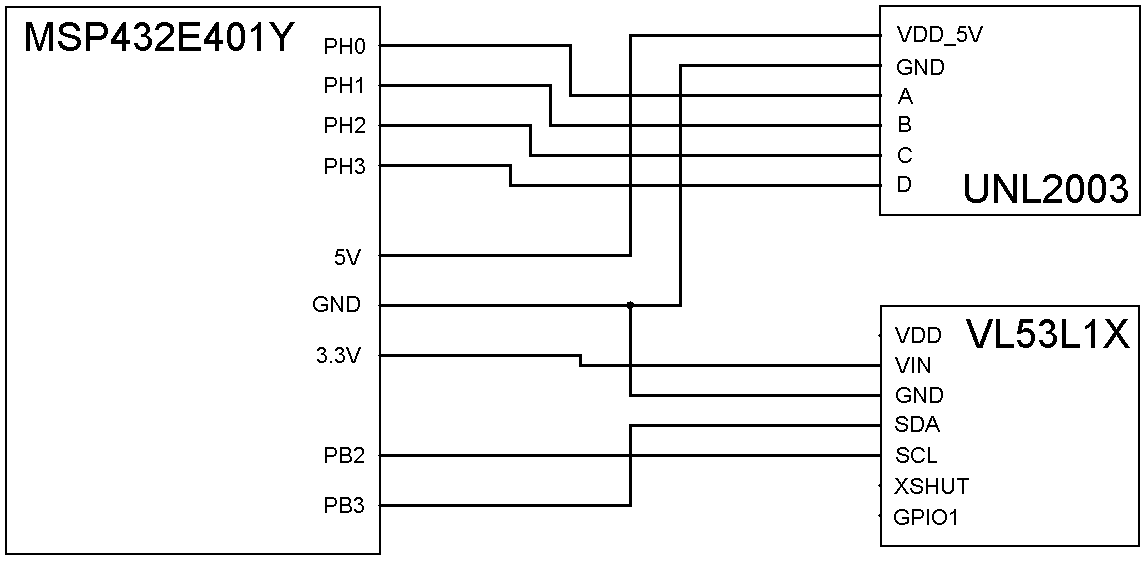
\includegraphics[width=\textwidth]{CircuitSchematic.png}
    \caption{Circuit Schematic}
    \label{fig:CircuitSchematic}
\end{figure}
\newpage
\section*{Programming Logic Flowchart}
\begin{figure}[h!]
    \centering
    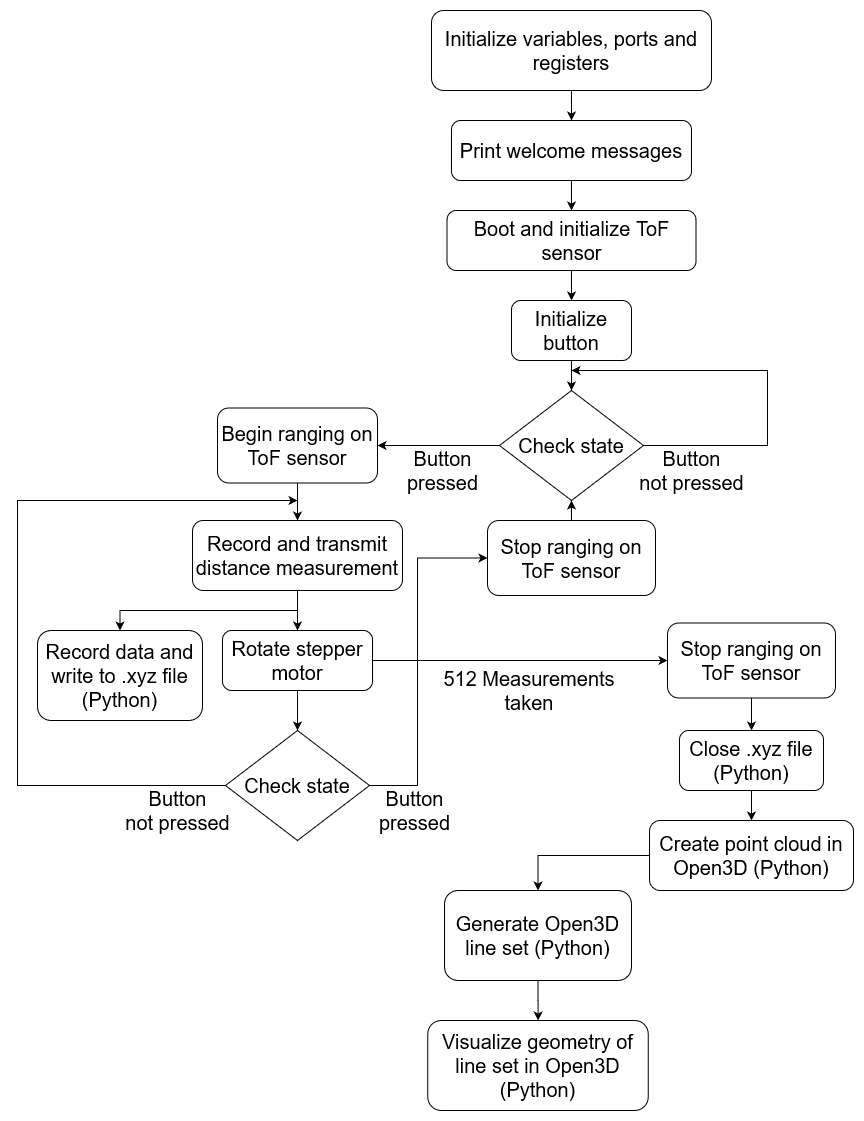
\includegraphics[width=0.95\textwidth]{FlowChart.png}
    \caption{Programming Logic Flowchart}
    \label{fig:Flowchart}
\end{figure}
\end{document}